\documentclass[11pt]{article}
\usepackage[margin=1in]{geometry}
\usepackage[T1]{fontenc}
\usepackage{lmodern}
\usepackage{graphicx,booktabs,microtype,caption,enumitem,xcolor}
\usepackage[colorlinks=true,linkcolor=black,citecolor=black,urlcolor=blue!60!black]{hyperref}
\captionsetup{font=small,labelfont=bf}
\setlist{itemsep=2pt,topsep=3pt}
\graphicspath{{figures/}}
\newcommand{\repo}[1]{\texttt{#1}}

\title{Reproducing and Improving FiDIP for Infant Pose Estimation on SyRIP}
\author{Nicholas Sheft \\ \small FiDIP hands-on exercise, report and repository}
\date{November 2026}

\begin{document}
\maketitle

\begin{abstract}
We reproduced the published FiDIP infant pose estimator and then tried to improve on it using the same SyRIP split and evaluation. The released FiDIP checkpoint reproduces exactly (Test100 AP 93.6). Retraining it from the shipped code does not: plain fine-tuning matches the paper (92.7), but FiDIP's domain-adaptation stage gives no gain over it (91.7). Our best system is Sapiens2-1B fine-tuned on the SyRIP training set. Over two seeds it reaches Test100 AP 95.4 and 95.3, and Test400 AP 94.2 and 94.3, against 90.7 for the released model. The gain comes from stronger pretraining, not from domain adaptation. We also report six changes that did not help, and show that the remaining errors are concentrated in occluded joints and unusual viewpoints.
\end{abstract}

\begin{table}[h]
\centering\small
\begin{tabular}{@{}ll@{}}
\toprule
Published baseline & DarkPose \cite{darkpose} (HRNet-W48 \cite{hrnet}) + FiDIP \cite{fidip}: SyRIP Test100 AP \textbf{93.6} \\
Our result & Sapiens2-1B fine-tuned: Test100 AP \textbf{95.4} / \textbf{95.3} (seeds 1 / 2) \\
Paired difference & $+1.75$ [$-0.04$, $+3.46$] and $+1.68$ [$+0.36$, $+3.18$] on Test100; \\
 & $+3.49$ [$+2.54$, $+4.60$] and $+3.54$ [$+2.66$, $+4.73$] on Test400 \\
Evaluation conditions & Official SyRIP split, COCO keypoint AP, ground-truth boxes, flip test \\
Checkpoint rule & Final epoch only; no test-based epoch selection for the reported model \\
\bottomrule
\end{tabular}
\caption{Summary of the claim. Brackets are 95\% paired bootstrap intervals (Section~\ref{sec:protocol}). Seed~1's Test100 interval touches zero, so Test400 is the stronger evidence.}
\label{tab:claim}
\end{table}

\section{Introduction}
Infant pose estimation matters for developmental monitoring, but labelled infant images are scarce and adult pose models transfer poorly. FiDIP \cite{fidip} addresses this by fine-tuning an adult model on SyRIP, a small set of real and synthetic infant images, with a domain classifier that pushes features to be invariant between real and synthetic data.

This project had three aims: rebuild the pipeline and reproduce the published numbers, evaluate carefully, and test whether the baseline can be improved under the same conditions. The main findings are:
\begin{itemize}
  \item The released model reproduces exactly, but FiDIP's advantage over plain fine-tuning does not reproduce from the shipped code (Section~\ref{sec:repro}).
  \item Stronger pretrained models help far more than any training change we tried. Sapiens2-1B gains $+3.5$ AP on Test400 over the released model (Section~\ref{sec:results}).
  \item One fine-tuned Sapiens2-1B is at least as good as our earlier two-model ensemble, under a non-inferiority test fixed before scoring.
  \item The official split has substantial source overlap between training and test images. Our gains hold on the images without such overlap.
\end{itemize}

\section{Data and evaluation protocol}
\label{sec:protocol}
\paragraph{Data.} SyRIP training data has 1200 images, 200 real and 1000 synthetic. Test100 is the published benchmark. Test500 is the larger labelled test set that contains it, and Test400 is the remaining 400 images. All results use the official split.

\paragraph{Metric.} COCO keypoint AP \cite{coco} with ground-truth person boxes and flip test. These are the conditions under which the released model reproduces the paper exactly.

\paragraph{Source overlap audit.} We compared training and test images by YouTube video id, perceptual hash and feature matching. 23 of the 25 training videos also supply test images. 147 Test400 images and 58 Test100 images have a direct link to a labelled training image, and six train/test pairs are near-identical. This overlap is in the original split and affects every model, including the baseline. We therefore also report \emph{Test400\_indep}, the 253 Test400 images with no such link.

\paragraph{Avoiding test-set tuning.} Early rounds, following the shipped code, selected the best epoch on Test100, which is optimistic. We label those numbers ``best'' and use them only to compare with the paper. All our improvement claims use final-epoch checkpoints. From round 12, new methods were screened by grouped 5-fold cross-validation on the 200 labelled real training images, with images from the same source kept in one fold. A method advanced only if pooled out-of-fold AP rose by at least 0.5 and at least 4 of 5 folds improved. Rules were written to \repo{PLAN.md} and committed before results were seen.

\paragraph{Uncertainty.} Paired bootstrap, 2000 resamples, resampling by source group so that related images are not treated as independent, with AP recomputed on each resample (\repo{scripts/bootstrap\_ap.py}).

\section{Reproducing FiDIP}
\label{sec:repro}
The FiDIP code runs on Python 3.12 and PyTorch 2.3.1, on a laptop (RTX 4060) with small Windows patches and on the Explorer cluster. Sapiens2 needs a separate environment (PyTorch 2.7.1, transformers 5.21). Table~\ref{tab:repro} compares our results with the paper. Both released checkpoints match exactly, on two machines for HRNet. The retrained plain fine-tune also matches. FiDIP itself does not.

\begin{table}[h]
\centering\small
\begin{tabular}{@{}lccc@{}}
\toprule
Test100 AP & Paper & Ours, best epoch & Ours, final epoch \\
\midrule
Released DarkPose + FiDIP & 93.6 & 93.6 & -- \\
Released Pose-MobileNet + FiDIP & 79.2 & 79.2 & -- \\
Retrained plain fine-tune (3 seeds) & 92.7 & 92.7 $\pm$ 0.2 & 92.3 $\pm$ 0.8 \\
Retrained FiDIP, code defaults (3 seeds) & 93.6 & 91.7 $\pm$ 0.4 & 90.9 $\pm$ 0.4 \\
\bottomrule
\end{tabular}
\caption{Reproduction. The released model also gives AP50 98.5, AP75 98.5 and AR 94.6, matching the paper.}
\label{tab:repro}
\end{table}

To find out why, we separated FiDIP's two ingredients (Table~\ref{tab:ablate}). The adversarial term alone is equivalent to fine-tuning. Pre-training the domain classifier costs about 1 AP on Test400. An early single run suggested BatchNorm drift during that stage was the cause, but freezing BatchNorm did not hold up over three seeds, so we rejected that explanation. We still cannot say why the released checkpoint beats everything we retrained with HRNet. The upstream README mentions a newer model trained on an expanded SyRIP, and we could not determine which model the released file is.

\begin{table}[h]
\centering\small
\begin{tabular}{@{}lccc@{}}
\toprule
HRNet-W48, 20 epochs & Seeds & Test400 (final) & Test100 (best) \\
\midrule
Plain fine-tune & 3 & 89.7 $\pm$ 0.4 & 92.7 $\pm$ 0.2 \\
Adversarial term only & 3 & 90.0 $\pm$ 0.3 & 92.5 $\pm$ 0.4 \\
Classifier pre-training only & 1 & 89.5 & 92.0 \\
Full FiDIP & 3 & 88.8 $\pm$ 0.5 & 91.7 $\pm$ 0.4 \\
Full FiDIP, BatchNorm frozen in pre-training & 3 & 88.2 $\pm$ 1.1 & 91.9 $\pm$ 0.6 \\
\midrule
Released FiDIP (reference) & -- & 90.7 & 93.6 \\
\bottomrule
\end{tabular}
\caption{Ablation of FiDIP's ingredients with the shipped code.}
\label{tab:ablate}
\end{table}

\section{Improving on the baseline}
\subsection{What we tried}
Table~\ref{tab:path} lists the main steps. Weight averaging (``soups'' \cite{soups}) gave small reliable gains. Moving to ViTPose++-H \cite{vitpose,vitposepp} gave a larger one, and fine-tuning it required a fix: its decoder BatchNorm layers misbehaved on small batches, which we solved by keeping them in evaluation mode. Sapiens2-1B \cite{sapiens2} scored 92.1 on Test400 with no infant training at all, and averaging its keypoints with ViTPose gave 94.0.

\begin{table}[h]
\centering\small
\begin{tabular}{@{}lcc@{}}
\toprule
System (final checkpoints) & Test400 & Test100 \\
\midrule
Released FiDIP (baseline) & 90.7 & 93.6 \\
HRNet-W48, 40-epoch fine-tune, 2 seeds & 90.2 $\pm$ 0.2 & 92.0 $\pm$ 0.5 \\
HRNet-W48 soup of four runs & 91.1 & 92.9 \\
ViTPose++-H zero-shot & 90.1 & 92.7 \\
ViTPose++-H fine-tuned (H20), 2 seeds & 92.8 $\pm$ 0.1 & 95.2 $\pm$ 0.2 \\
ViTPose++-H soup of two seeds (D-soup) & 93.1 & 95.7 \\
Sapiens2-1B zero-shot & 92.1 & 93.4 \\
D-soup + Sapiens2-1B zero-shot, 0.5/0.5 keypoint average & 94.0 & 95.4 \\
\textbf{Sapiens2-1B fine-tuned, seeds 1 / 2} & \textbf{94.2 / 94.3} & \textbf{95.4 / 95.3} \\
\bottomrule
\end{tabular}
\caption{Path from the baseline to the final system.}
\label{tab:path}
\end{table}

Several ideas did not help, and we report them as results:
\begin{itemize}
  \item \textbf{Recipe changes on ViTPose++-H:} layer-wise learning-rate decay, 384$\times$288 input and different real:synthetic mixes all landed at Test400 92.6--93.0.
  \item \textbf{Synthetic data:} training on the 200 real images alone also gave Test400 92.8 $\pm$ 0.1, though Test100 fell to 94.6 $\pm$ 0.2. For a strong backbone, synthetic data adds nothing measurable on Test400.
  \item \textbf{Ranking loss (RSPose \cite{rspose}):} $-0.36$ pooled cross-validation AP, better in 1 of 5 folds.
  \item \textbf{Mean-teacher self-training} \cite{meanteacher} on the 52 unlabelled images with no link to the test set: $-0.78$, better in 0 of 5 folds.
  \item \textbf{Correcting training labels:} a human-reviewed audit fixed 18 joints in 16 images, and 0 of 20 random control images had errors. The effect was $-0.11$, within noise. Label noise at this level (about 0.6\% of real joints) is not the limit.
\end{itemize}

\subsection{Final method: fine-tuning Sapiens2-1B}
We fine-tune all weights of \repo{facebook/sapiens2-pose-1b} (\repo{tools/train\_sapiens2.py}). The pretrained 308-keypoint head is kept. The 17 COCO joints are written into their matching channels and the loss uses only those channels, so no new head is learned. Crops and Gaussian heatmap targets come from the model's own processor (1024$\times$768 input, 256$\times$192 heatmaps, $\sigma=6$), so training targets match what its decoder inverts. Converting targets back to coordinates gave 0.000\% error before training, plain and flipped.

Training uses AdamW (learning rate $10^{-5}$, weight decay 0.01), batch size 8, bf16 and gradient checkpointing, for 10 epochs with the learning rate cut tenfold from epoch 8. Augmentation is horizontal flip, box scale 0.75--1.25, box shift $\pm$0.1 and colour jitter 0.3. The recipe was fixed before any fine-tuned score was seen, with the epoch count chosen to match the step count of the ViTPose recipe. Each run takes about 1.4 hours on one A100 80GB and uses 38\,GB.

\section{Results}
\label{sec:results}
\subsection{Comparison with the baseline}
Figure~\ref{fig:headline} compares each system with the released model on the same images. The HRNet models we trained stay at or below the baseline. Both fine-tuned Sapiens2 seeds clearly beat it on Test400, and by more on the images with no source overlap ($+4.0$ and $+4.1$), so the gain is not explained by train/test overlap. Test100 has only 100 images, so its intervals are wide.

\begin{figure}[t]
\centering
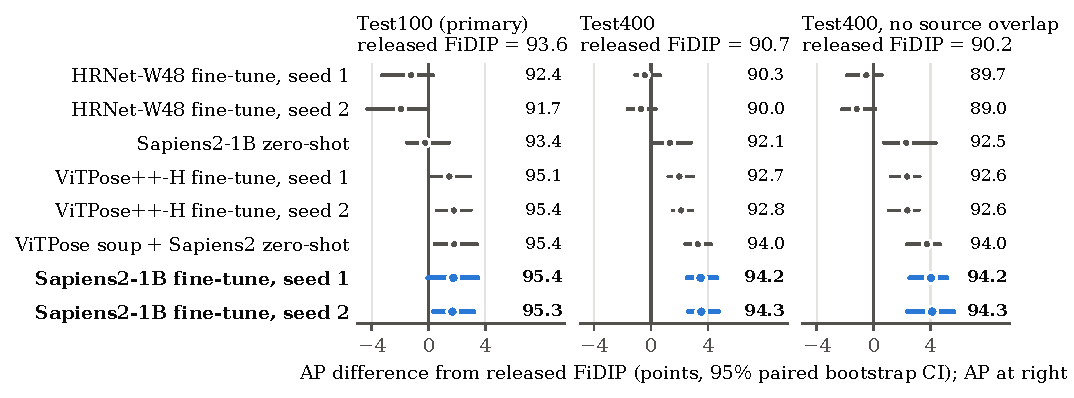
\includegraphics[width=\linewidth]{fig_headline}
\caption{Paired AP difference from the released FiDIP model, with 95\% source-group bootstrap intervals. Numbers at right are absolute AP. All systems use final checkpoints.}
\label{fig:headline}
\end{figure}

\subsection{Controlled comparisons}
Table~\ref{tab:cv} gives the cross-validation result, where every system is scored on real images it did not train on. Fine-tuning accounts for $+1.34$ AP with the architecture, data and evaluation unchanged, and is better in 5 of 5 folds. On the test sets the same comparison gives $+2.2$ on Test400. Scores on the corrected labels rank the systems the same way.

\begin{table}[h]
\centering\small
\begin{tabular}{@{}lcc@{}}
\toprule
Pooled out-of-fold AP, 200 real images & Original labels & Corrected labels \\
\midrule
ViTPose++-H (H20) & 94.39 & 94.95 \\
Sapiens2-1B zero-shot & 94.76 & 94.88 \\
H20 + Sapiens2 zero-shot & 95.94 & 96.38 \\
H20 + Sapiens2 fine-tuned & 96.05 & 96.40 \\
\textbf{Sapiens2-1B fine-tuned} & \textbf{96.10} & \textbf{96.41} \\
\bottomrule
\end{tabular}
\caption{Grouped 5-fold cross-validation. Fine-tuned folds on original labels: 94.3, 96.3, 97.3, 96.5, 96.2.}
\label{tab:cv}
\end{table}

Our pre-registered test asked whether adding the fine-tuned model to H20 beat the zero-shot ensemble by at least 0.5. It did not ($+0.10$, 2 of 5 folds), so the ensemble was not advanced. The fine-tuned model alone, however, matched the ensemble, which raised a second question: can it replace two models with one? We fixed a non-inferiority test before scoring: for both seeds, the Test400 lower bound of the difference from D-soup + zero-shot Sapiens2 must exceed $-0.5$. Both passed, at $+0.20$ [$-0.10$, $+0.67$] and $+0.25$ [$-0.15$, $+0.88$]. The single model is at least as good, not shown to be better. Adding D-soup back gives no further gain (Test400 94.2 and 94.0). This second test is exploratory.

\subsection{Repeatability}
The two seeds differ by at most 0.1 AP on each set. Their per-image OKS scores correlate at 0.99, and 21 of each seed's 25 worst images are shared.

\section{Successes and failure cases}
\label{sec:failure}
We analysed Test500 predictions per joint and per image (\repo{scripts/failure\_analysis.py}). A joint counts as \emph{missed} when its COCO similarity score is below 0.5.

\paragraph{No photographs, by choice.} This report deliberately shows no SyRIP photographs. They are images of infants from a password-protected dataset, so failure cases are drawn as skeletons instead. We did inspect the images themselves privately, and the descriptions below come from that inspection. The skeleton figure is also kept out of the repository because it contains label coordinates. It appears only in the submitted PDF, and \repo{scripts/make\_report\_figures.py} rebuilds it for anyone with SyRIP access.

\paragraph{Where the gain comes from.} Figure~\ref{fig:joints} shows that the improvement is broad, and largest at the wrists, knees and ankles. Across Test500, images with OKS below 0.85 fall from 42 to 21. Left/right confusions on Test400 fall from 43 joint pairs to 23, but ViTPose (23) and zero-shot Sapiens2 (22) reach the same level, so that gain comes from stronger pretrained models rather than from fine-tuning.

\begin{figure}[t]
\centering
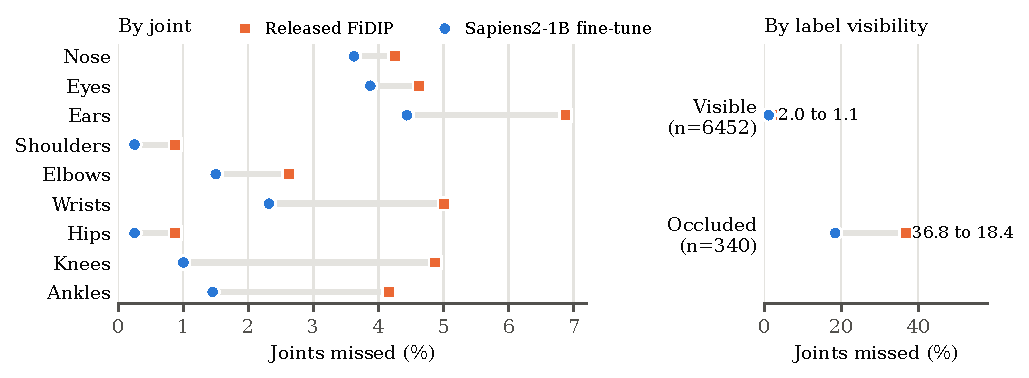
\includegraphics[width=\linewidth]{fig_joints}
\caption{Share of labelled joints missed on Test400, for the released model and the fine-tuned model (mean of two seeds). Left and right joints are pooled.}
\label{fig:joints}
\end{figure}

\paragraph{Occlusion is the main remaining problem.} Occluded joints are 5\% of labelled Test400 joints but about half of all misses, for both models (49\% released, 46\% fine-tuned seed~1). Fine-tuning halves their miss rate from 36.8\% to 18.4\%, yet they remain far harder than visible joints (1.1\%). This also helps explain why Test100 scores run higher: only 13 of its 1700 labelled joints (0.8\%) are marked occluded.

\paragraph{Viewpoint and posture.} We inspected the 12 images with the lowest OKS. Five show a crawling or sitting infant seen from behind or the side, with hips and legs overlapping, and appear to come from just two scenes. Four are head-first, upside-down or curled views. Two have the body hidden by a toy or clothing. Figure~\ref{fig:skeletons} shows examples. Posture labels exist only for Test100 (Table~\ref{tab:posture}). The model improves on supine and prone infants, the two large groups, while prone stays slightly harder by mean OKS. Sitting and standing have too few images to interpret.

\begin{table}[h]
\centering\small
\begin{tabular}{@{}lcccc@{}}
\toprule
Test100 AP & Supine (43) & Prone (41) & Sitting (11) & Standing (5) \\
\midrule
Released FiDIP & 92.1 & 93.8 & 93.6 & 100.0 \\
Sapiens2-1B fine-tuned, seed 1 & 94.3 & 95.2 & 96.8 & 100.0 \\
Sapiens2-1B fine-tuned, seed 2 & 94.5 & 95.2 & 94.5 & 100.0 \\
\bottomrule
\end{tabular}
\caption{AP by posture, with image counts in brackets.}
\label{tab:posture}
\end{table}

\begin{figure}[t]
\centering
\IfFileExists{figures/fig_skeletons.pdf}{\includegraphics[width=\linewidth]{fig_skeletons}}{\fbox{\parbox{.95\linewidth}{\centering\small Figure not in the repository: it contains SyRIP label coordinates. See the submitted PDF.}}}
\caption{Skeletons from six Test500 images. Top row: cases the fine-tuned model corrects. Bottom row: remaining failures. Bottom right: the four different models we compared agree with each other (mean pairwise OKS 0.98) but not with the label (OKS about 0.09), which points to a label error. Photographs are deliberately omitted (see Section~\ref{sec:failure}).}
\label{fig:skeletons}
\end{figure}

\paragraph{Regressions.} The fine-tuned model is not uniformly better. On image 277, for example, OKS falls from 0.71 to 0.62 (Figure~\ref{fig:skeletons}, bottom left).

\paragraph{Some ``failures'' are label problems.} Image 149 is the clearest case. Removing that one image raises Test400 AP by 0.18 for the released model and by about 0.4 for the fine-tuned model. We left the test labels unchanged. On three further low-scoring images (165, 171 and 367), the models agree closely with each other (mutual OKS at least 0.91) while 5 to 9 joints are labelled occluded. There, labels and models may simply be guessing differently about hidden joints, and we cannot say which is right.

\section{Limitations}
\begin{itemize}
  \item \textbf{Different model, not a better FiDIP.} Our gain comes from a much larger model with far broader pretraining, reported as about one billion human images \cite{sapiens2docs}. It says nothing against domain adaptation in principle, and it costs more at inference (1024$\times$768 input, about 1B parameters).
  \item \textbf{Test sets were reused.} Test400 informed earlier method choices, including the decision to pursue Sapiens2. The final recipe was fixed without test scores, but model-family selection was not blind, so the test results are supporting evidence rather than a clean confirmation.
  \item \textbf{Possible leakage we cannot rule out.} SyRIP's real images come from public web sources. We did not audit Sapiens2's pretraining data, and an overlap there would not be caught by Test400\_indep.
  \item \textbf{Small samples.} Test100 cannot separate our top systems, the posture groups are small, and two seeds show consistency rather than a full distribution.
  \item \textbf{Ground-truth boxes.} All numbers assume a perfect person box, so a deployed system would score lower.
  \item \textbf{Unexplained baseline.} We could not retrain a model that matches the released checkpoint.
\end{itemize}

\section{Lessons learned}
\begin{itemize}
  \item Reproducing a checkpoint and reproducing a method are different. The first succeeded exactly and the second did not.
  \item Single runs mislead. The BatchNorm explanation looked convincing at one seed and failed at three.
  \item Pretraining dominated on this small dataset. Every training-recipe change we tried on a strong backbone was within noise.
  \item Writing the decision rule first kept us honest. Most of our later ideas failed it, and the rule stopped us from promoting them.
  \item A split can hide leakage. Auditing sources changed how we read every later result.
  \item Inference-ready models may need checks before training. Comparing train-mode and eval-mode loss on one batch would have found the ViTPose BatchNorm problem at once.
\end{itemize}

\section{Reproducibility}
\repo{MANIFEST.md} starts with the final system's exact commands, environments, checkpoints and job IDs. \repo{results/} holds all scores, failure-analysis tables, bootstrap outputs and training logs, and \repo{scripts/make\_report\_figures.py} rebuilds the figures. The final model is trained with:
\begin{verbatim}
sbatch -J fidip-full-s2ft-s1 --gres=gpu:a100:1 --constraint=a100@80g \
  --time=02:30:00 scripts/sapiens2_ft.sbatch full-s2ft-s1 all \
  --epochs 10 --seed 1 --save
\end{verbatim}
SyRIP is password-protected, so the data, derived annotations and prediction files are not in the repository. The reported scores come from predictions written at the end of each training job, by the trained model in memory. \repo{scripts/sapiens2\_eval.sbatch} repeats the Test500 prediction from the saved weights in a separate job. We ran it for both seeds on V100 GPUs, whereas the original predictions came from A100s, so exact equality was not expected. Test100 and Test400 AP each changed by about 0.01 points or less for both seeds. The pooled 500-image AP changed by $-0.09$ (seed 1) and $+0.01$ (seed 2). The median joint moved 0.06 pixels. Of the 8{,}500 joints per seed, 3 and 2 moved more than 5 pixels, at most 38.8, and all of those had confidence below 0.65. The saved weights therefore reproduce the reported Test100 and Test400 scores.

\section{Use of AI tools}
This was an agentic project, as the assignment requires. Claude Code worked with the author throughout. It set up environments, wrote and ran code and cluster jobs, kept \repo{AGENT.md}, \repo{SKILL.md} and \repo{MANIFEST.md}, ran the literature search, and drafted this report. The author set the research direction, wrote the round 12 plan, chose which experiments to pursue, adjudicated every flagged label by hand, and reviewed the results.

AI-assisted work needed checking. Examples logged in \repo{AGENT.md} include a misread training-log column, a label-correction tool that first applied swaps it should have skipped, and concurrent jobs that lost rows from a shared results file. Each was caught from the logs and fixed before results were used. All numbers in this report were taken from logged outputs.

\begin{thebibliography}{99}\small
\bibitem{fidip} X.~Huang, N.~Fu, S.~Liu, and S.~Ostadabbas. Invariant representation learning for infant pose estimation with small data. In \emph{IEEE International Conference on Automatic Face and Gesture Recognition (FG)}, 2021.
\bibitem{coco} T.-Y.~Lin et al. Microsoft COCO: Common objects in context. In \emph{ECCV}, 2014.
\bibitem{soups} M.~Wortsman et al. Model soups: Averaging weights of multiple fine-tuned models improves accuracy without increasing inference time. In \emph{ICML}, 2022.
\bibitem{vitpose} Y.~Xu, J.~Zhang, Q.~Zhang, and D.~Tao. ViTPose: Simple vision transformer baselines for human pose estimation. In \emph{NeurIPS}, 2022.
\bibitem{vitposepp} Y.~Xu, J.~Zhang, Q.~Zhang, and D.~Tao. ViTPose++: Vision transformer for generic body pose estimation. \emph{IEEE TPAMI}, 2024.
\bibitem{sapiens2} R.~Khirodkar, H.~Wen, J.~Martinez, Y.~Dong, Z.~Su, and S.~Saito. Sapiens2. arXiv:2604.21681, 2026.
\bibitem{sapiens2docs} Hugging Face. Sapiens2 model documentation. \url{https://huggingface.co/docs/transformers/model_doc/sapiens2}.
\bibitem{hrnet} K.~Sun, B.~Xiao, D.~Liu, and J.~Wang. Deep high-resolution representation learning for human pose estimation. In \emph{CVPR}, 2019.
\bibitem{darkpose} F.~Zhang, X.~Zhu, H.~Dai, M.~Ye, and C.~Zhu. Distribution-aware coordinate representation for human pose estimation. In \emph{CVPR}, 2020.
\bibitem{rspose} M.~C.~Kele\c{s}, B.~Cetinkaya, S.~Kalkan, and E.~Akba\c{s}. RSPose: Ranking based losses for human pose estimation. arXiv:2511.13857, 2025.
\bibitem{meanteacher} A.~Tarvainen and H.~Valpola. Mean teachers are better role models. In \emph{NeurIPS}, 2017.
\end{thebibliography}

\end{document}
